To PiLock αποτελείται από 2 κύρια μέρη: Τον εξυπηρετητή (Server) και τον πελάτη (Client).

\section{Σύντομη Περιγραφή Λογισμικού Εξυπηρετητή - PiLock Server}
	Ο εξυπηρετητής αποτελείται από το Hardware που χρειάζεται προκειμένου να λειτουργήσει το PiLock, καθώς επίσης και το αντίστοιχο λογισμικό υπεύθυνο για την διαχείρηση της κλειδαριάς, από όλες τις απόψεις. Πιο συγκεκριμένα, το λογισμικό είναι υπεύθυνο για:
	\begin{itemize}
		\item Την διαχείριση του Hardware υπεύθυνου για την λειτουργία του μηχανισμού ξεκλειδώματος.
		\item Την αυθεντικοποίηση των ήδη υπάρχοντων χρηστών.
		\item Την δημιουργία νέων χρηστών, ικανών για αυθεντικοποίηση (εξουσιοδοτημένοι χρήστες).
		\item Την τήρηση ιστορικού αυθεντικοποιήσεων (επιτυχών ή μή).
	\end{itemize}
	Το λογισμικό του εξυπηρετητή αναλύεται πλήρως στην αντίστοιχη ενότητα. %TODO FIX IT

\section{Σύντομη Περιγραφή Λογισμικού Πελάτη - PiLock Client}
	Η πλευρά του πελάτη αποτελείται από την εφαρμογή του PiLock, σχεδιασμένη για κινητά που τρέχουν Android, καθώς επίσης και από την εφαρμογή σχεδιασμένη για Android Wear Smartwatches.

	Πιο συγκεκριμένα, οι εφαρμογές στο πεδίο του πελάτη είναι υπεύθυνες για:

	\begin{itemize}
		\item Σύνδεση στην πλατφόρμα του PiLock\textsuperscript{*}.
		\item Αποστολή αιτημάτων ξεκλειδώματος.
		\item Αποστολή αιτημάτων αλλαγής PIN\textsuperscript{*}.
	\end{itemize}
	{\footnotesize Οι δυνατότητες που είναι σημειωμένες με τον αστερίσκο (*) είναι διαθέσιμες αποκλειστικά στην εφαρμογή για κινητά (mobile app) και όχι στην εφαρμογή για Android Wear.}

\section{Υλικό - Hardware}
	Όπως αναφέραμε και στην εισαγωγή, ένας εκ των στόχων από τις πρώτες μέρες του σχεδιασμού του PiLock ήταν να υλοποιηθεί το Project με όσο το δυνατόν λιγότερο κόστος. Προκειμένου αυτό να είναι εφικτό, χρησιμοποιήσαμε υλικό εύκολα προσκομίσιμο και, όπου ήταν δυνατόν, Open Source Hardware.

	"Εγκέφαλος" όλης της κατασκευής είναι το Raspberry Pi Zero W (RPi Zero W), ένας υπολογιστής μοναδικής πλακέτας (Single Board). Σχεδιάζεται από το Raspberry Pi Foundation στην Αγγλία και η κυκλοφορία του ξεκίνησε τον Φεβρουάριο του 2017. Σκοπός του RPi Zero W είναι να συμπληρώσει το προηγούμενο μοντέλο, το Raspberry Pi Zero, φέρνοντας δυνατότητες συνδεσιμότητας WiFi 802.11n και BlueTooth 4.0 χωρίς Hardware κάποιου τρίτου (μέχρι προτίστως έπρεπε να χρησιμοποιηθεί κάποιο WiFi ή BlueTooth Dongle προκειμένου να υπάρξει αυτή η συνδεσιμότητα) \cite{rpizw}.

	\begin{figure}[h]
		\centering
			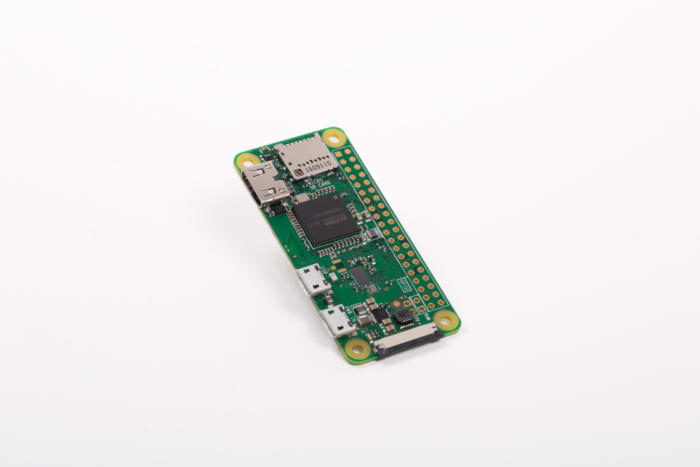
\includegraphics[width=\textwidth,height=\textheight,keepaspectratio]{rpizerow.jpg}
		\caption{Το Raspberry Pi Zero W.}
	\end{figure}

	Στην "καρδιά" του RPi Zero W υπάρχει ένας Broadcom BCM2835, 32-bit επεξεργαστής αρχιτεκτονικής ARMv6, χρονισμένος στο 1Ghz. Για μνήμη τυχαίας προσπέλασης χρησιμοποιούνται 512MB Low Power Double Data Rate 2 (LPDDR2) RAM. 
